% !TEX program = xelatex
\documentclass[12pt,a4paper]{ctexart}

% ==================== Packages ====================
\usepackage{amsmath,amssymb,amsfonts}
\usepackage{graphicx}
\usepackage{geometry}
\usepackage{setspace}
\usepackage{enumitem}
\usepackage{booktabs}
\usepackage{float}
\usepackage{array}
\usepackage[table]{xcolor}
\usepackage{listings}
\usepackage{caption}
\usepackage{subcaption}
\usepackage{hyperref}
\usepackage{multirow}
\usepackage{makecell}

% ==================== 代码块样式 ====================
\lstset{
    language=Python,
    basicstyle=\footnotesize\ttfamily,
    keywordstyle=\color{blue}\bfseries,
    commentstyle=\color{gray!60!black},
    stringstyle=\color{red!70!black},
    numbers=left,
    numberstyle=\scriptsize\color{gray!50},
    stepnumber=1,
    numbersep=6pt,
    frame=single,
    breaklines=true,
    breakatwhitespace=false,
    showstringspaces=false,
    tabsize=4,
    captionpos=b,
    aboveskip=8pt,
    belowskip=6pt,
    columns=flexible,
    keepspaces=true
}

% ==================== 页面设置 ====================
\geometry{margin=0.95in}
\onehalfspacing
\setlength{\parskip}{2pt plus 1pt minus 1pt}

% ==================== 标题 ====================
\title{\textbf{毫米波雷达 FMCW 测距测速仿真与目标分类}\\[0.4cm]
\large 智能感知技术课程大作业}
\author{西安科技大学 \ 通信与信息工程学院 \ 电子科学与技术专业 \\
姓名：张凯文 \quad 学号：25207035001}
\date{\today}

\begin{document}

\maketitle

% ==================== 摘要 ====================
\begin{abstract}
\noindent
本报告分为两个部分。第一部分基于 FMCW（调频连续波）毫米波雷达的工作原理，在 MATLAB 程序的基础上，使用 Python 复现了测距与测速仿真。在原始单个目标（距离 32 m，速度 28.12 m/s）的基础上，新增两个不同距离和速度的目标（目标2：距离 60 m，速度 12.50 m/s；目标3：距离 85 m，速度 50.00 m/s），通过距离维 FFT 和二维 FFT（距离-多普勒处理）成功分离了三个目标的距离与速度信息。第二部分基于实测雷达数据，采用 SVM、决策树、随机森林等机器学习方法对金杯（小型车）、厢式货车（大型车）和无人机三类目标进行分类识别，轨迹点级最高准确率达 98.10\%，文件级（航迹级）最高准确率达 94.44\%。

\noindent \textbf{关键词：} FMCW 雷达，测距测速，距离-多普勒，目标分类，SVM，随机森林，机器学习。
\end{abstract}

% ==================== 第一部分：FMCW 仿真 ====================
\section{FMCW 毫米波雷达测距测速仿真}

\subsection{FMCW 雷达工作原理}

调频连续波（Frequency Modulated Continuous Wave, FMCW）雷达通过发射频率随时间线性变化的信号（啁啾信号），并接收目标反射的回波信号。由于回波信号相对于发射信号存在时间延迟 $\tau = 2R/c$（$R$ 为目标距离，$c$ 为光速），混频后得到的差频信号频率 $f_b$ 与目标距离成正比：
\begin{equation}
    f_b = K \cdot \tau = K \cdot \frac{2R}{c} = \frac{B}{T} \cdot \frac{2R}{c}
\end{equation}
其中 $K = B/T$ 为调频斜率，$B$ 为信号带宽，$T$ 为啁啾周期。因此，通过对差频信号进行 FFT（距离维 FFT），可在频谱中定位目标的距离信息。

对于运动目标，其回波信号还会产生多普勒频移 $f_d = 2v f_0 / c$（$v$ 为目标径向速度，$f_0$ 为载频）。通过发射多个周期的啁啾信号，对慢时间维进行第二次 FFT（多普勒维 FFT），即可提取目标的速度信息。这种距离-多普勒二维 FFT 处理是 FMCW 雷达的核心信号处理流程。

\subsection{系统参数设置}

仿真采用以下雷达系统参数，与原始 MATLAB 程序保持一致：

\begin{table}[H]
\centering
\caption{雷达系统参数}
\begin{tabular}{lll}
\toprule
\textbf{参数名称} & \textbf{符号} & \textbf{数值} \\
\midrule
光速           & $c$      & $3 \times 10^8$ m/s \\
载频           & $f_0$    & 24 GHz \\
信号带宽       & $B$      & 150 MHz \\
啁啾周期       & $T$      & 20 $\mu$s \\
调频斜率       & $K$      & $7.5 \times 10^{12}$ Hz/s \\
啁啾个数       & $N_{\text{chirp}}$ & 50 \\
采样频率       & $f_s$    & 500 MHz \\
每周期采样点数 & $N_f$    & 10000 \\
总采样点数     & $N$      & 500000 \\
\midrule
距离分辨率     & $\Delta R = c/(2B)$      & 1 m \\
最大探测距离   & $R_{\max} = c f_s/(2K)$   & 约 200 m \\
速度分辨率     & $\Delta v = c/(2 f_0 T N_{\text{chirp}})$ & 约 0.125 m/s \\
\bottomrule
\end{tabular}
\end{table}

\subsection{目标参数}

原始程序中仅包含一个目标。本作业要求额外添加两个速度、距离均不同的目标，三目标的参数如下：

\begin{table}[H]
\centering
\caption{三目标参数设置}
\begin{tabular}{cccc}
\toprule
\textbf{目标编号} & \textbf{初始距离 (m)} & \textbf{径向速度 (m/s)} & \textbf{多普勒频移 (kHz)} \\
\midrule
目标1（原始） & 32  & 28.12 & 4.5  \\
目标2（新增） & 60  & 12.50 & 2.0  \\
目标3（新增） & 85  & 50.00 & 8.0  \\
\bottomrule
\end{tabular}
\end{table}

\subsection{信号处理流程}

信号处理流程主要包括以下步骤：

\begin{enumerate}[leftmargin=*, label=步骤\arabic*:]
    \item \textbf{发射信号生成：} 对每个啁啾周期，生成本地线性调频信号 $s_t(t) = \exp\left[j 2\pi \left(f_0 t + \frac{1}{2}K t^2\right)\right]$，并通过矩形窗截取有效区间。
    \item \textbf{回波信号建模：} 对每个目标，根据其时变距离 $R(t) = R_0 - v t$ 计算时延 $\tau(t) = 2R(t)/c$，生成延迟后的回波信号。三目标的回波信号叠加构成总接收信号。
    \item \textbf{混频（去斜）：} 将接收信号与发射信号的共轭相乘 $s_{\text{mix}}(t) = s_r(t) \cdot s_t^*(t)$，得到差频信号。
    \item \textbf{距离维 FFT：} 将差频信号重构为快时间-慢时间矩阵（$50 \times 10000$），沿快时间维进行 10000 点 FFT，得到目标的距离信息。
    \item \textbf{二维 FFT（距离-多普勒）：} 对矩阵进行二维 FFT（$100 \times 10000$ 点），同时获取距离和速度（多普勒频率）信息。
\end{enumerate}

\subsection{仿真结果与分析}

\subsubsection{差频信号}

图 \ref{fig:beat} 展示了第一个啁啾周期混频后的差频信号实部。由于存在三个不同距离的目标，差频信号中包含三个不同频率分量的叠加。

\begin{figure}[H]
    \centering
    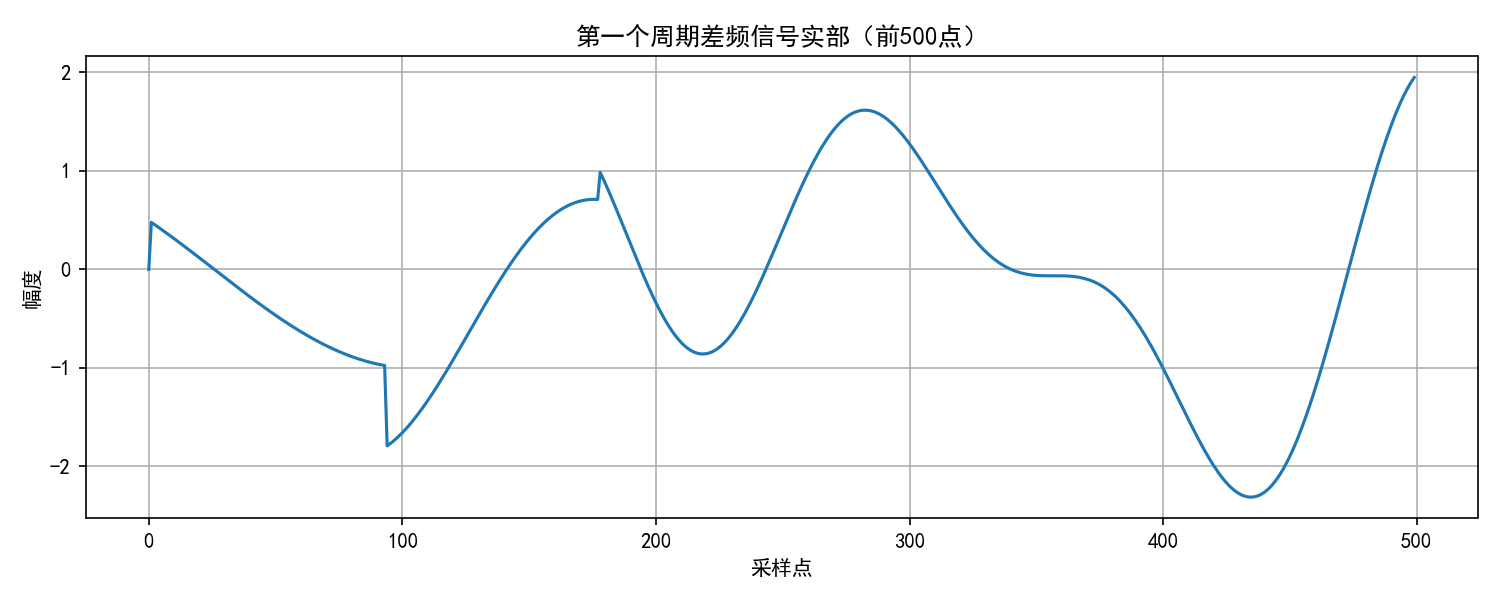
\includegraphics[width=0.85\textwidth]{fig3_beat_signal.png}
    \caption{第一个周期差频信号实部（前500采样点）}
    \label{fig:beat}
\end{figure}

\subsubsection{距离维 FFT}

图 \ref{fig:range_fft} 为距离维 FFT 后的三维网格图，横轴为距离，纵轴为啁啾周期编号。可以清晰地看到三个峰值，分别位于约 32 m、60 m 和 85 m 处，与预设的三目标距离完全吻合。

\begin{figure}[H]
    \centering
    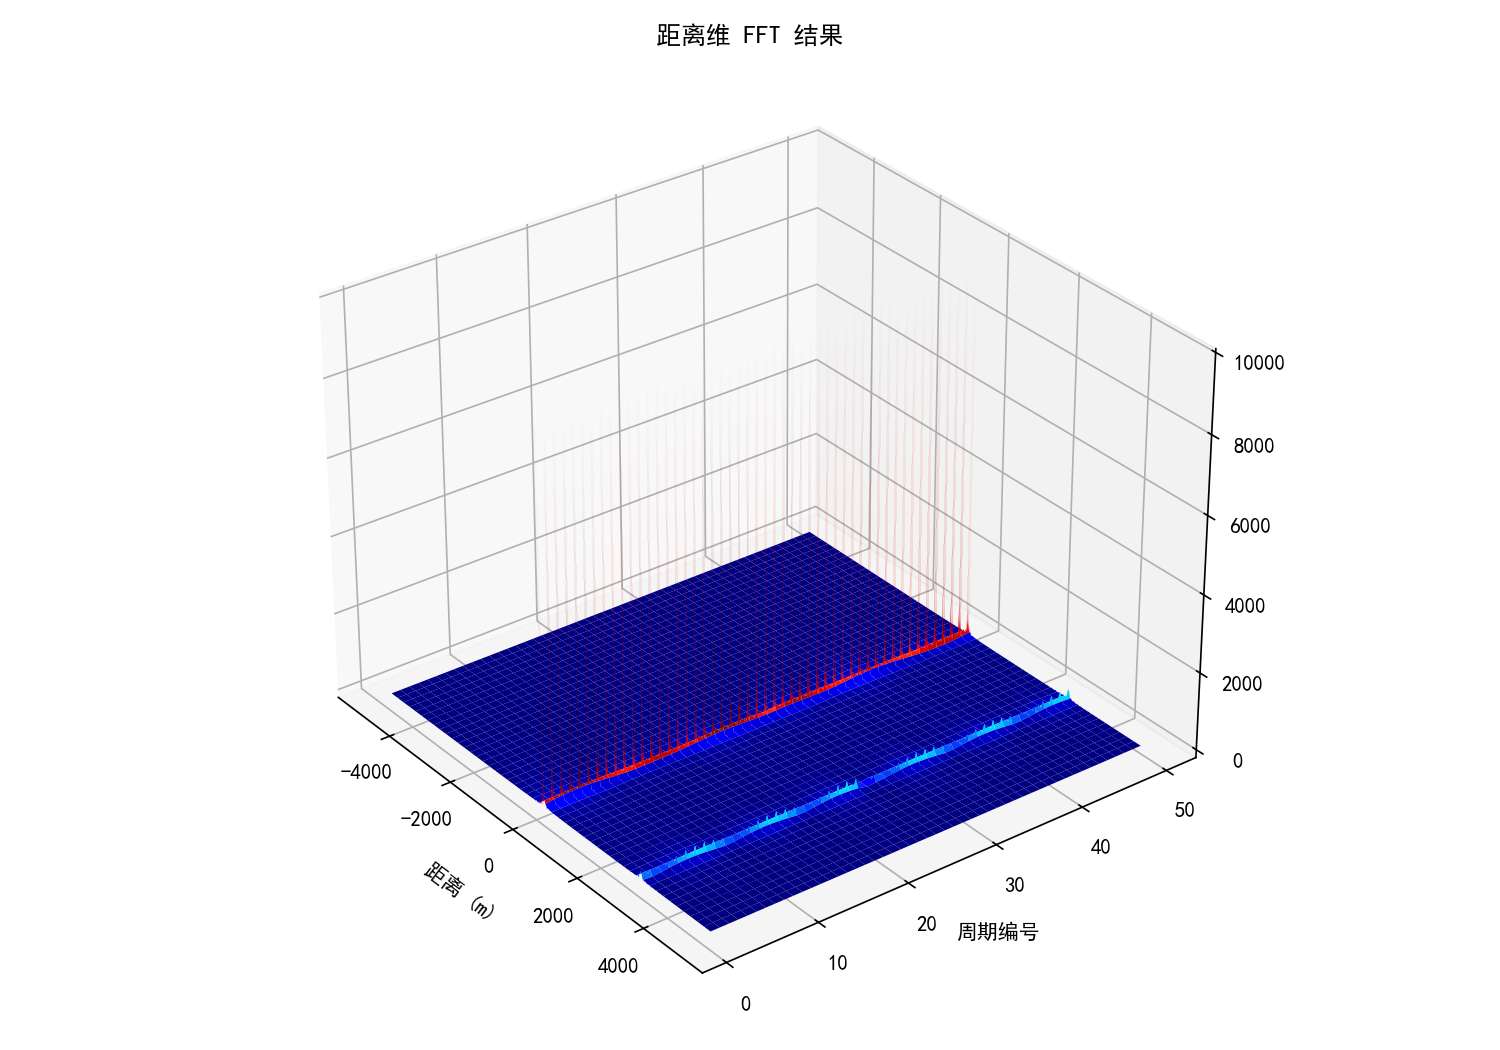
\includegraphics[width=0.85\textwidth]{fig4_range_fft_mesh.png}
    \caption{距离维 FFT 三维网格图}
    \label{fig:range_fft}
\end{figure}

图 \ref{fig:range_slice} 为第一个啁啾周期在距离维上的切片图，三个目标的距离峰值清晰可辨，峰值位置与预设参数一致。

\begin{figure}[H]
    \centering
    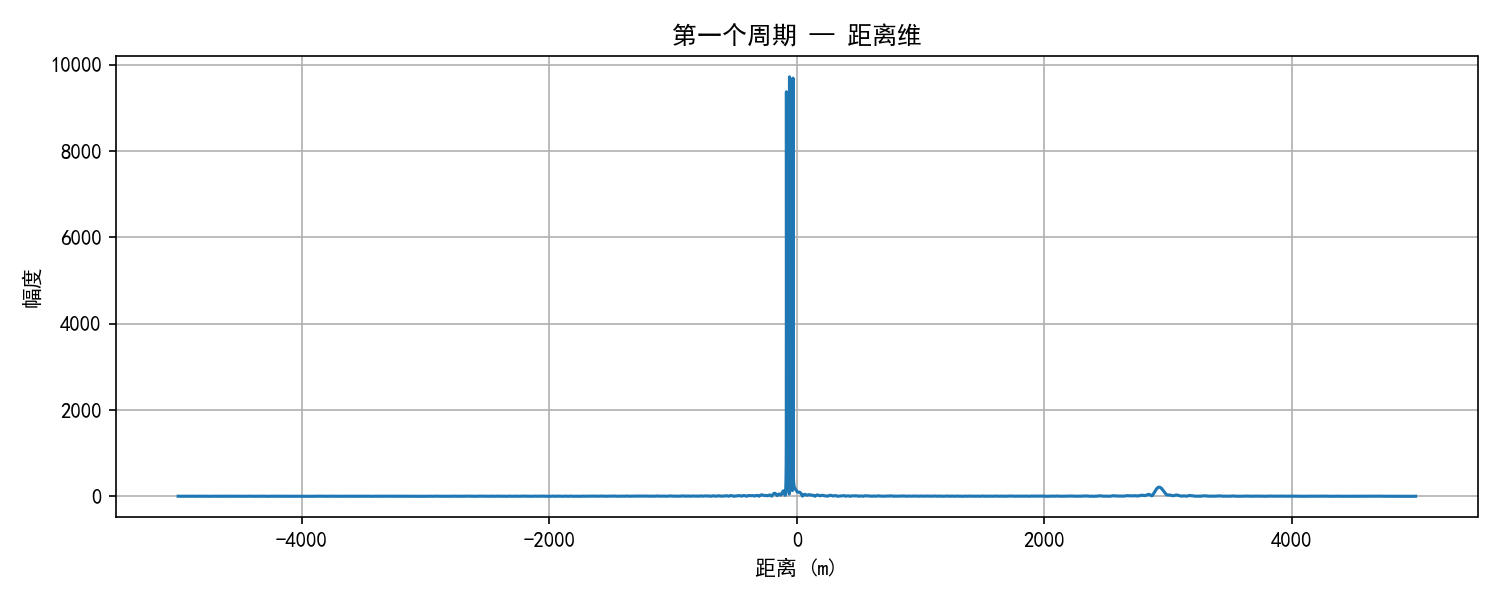
\includegraphics[width=0.85\textwidth]{fig6_range_slice.png}
    \caption{第一个周期——距离维切片}
    \label{fig:range_slice}
\end{figure}

\subsubsection{距离-多普勒二维 FFT}

图 \ref{fig:rd_map} 为距离-多普勒二维 FFT 结果的三维网格图。三个目标在距离-速度平面上形成三个独立的峰值点，分别对应：
\begin{itemize}[leftmargin=*]
    \item 目标1：距离 32 m，多普勒频率约 4.5 kHz（速度 28.12 m/s）
    \item 目标2：距离 60 m，多普勒频率约 2.0 kHz（速度 12.50 m/s）
    \item 目标3：距离 85 m，多普勒频率约 8.0 kHz（速度 50.00 m/s）
\end{itemize}

\begin{figure}[H]
    \centering
    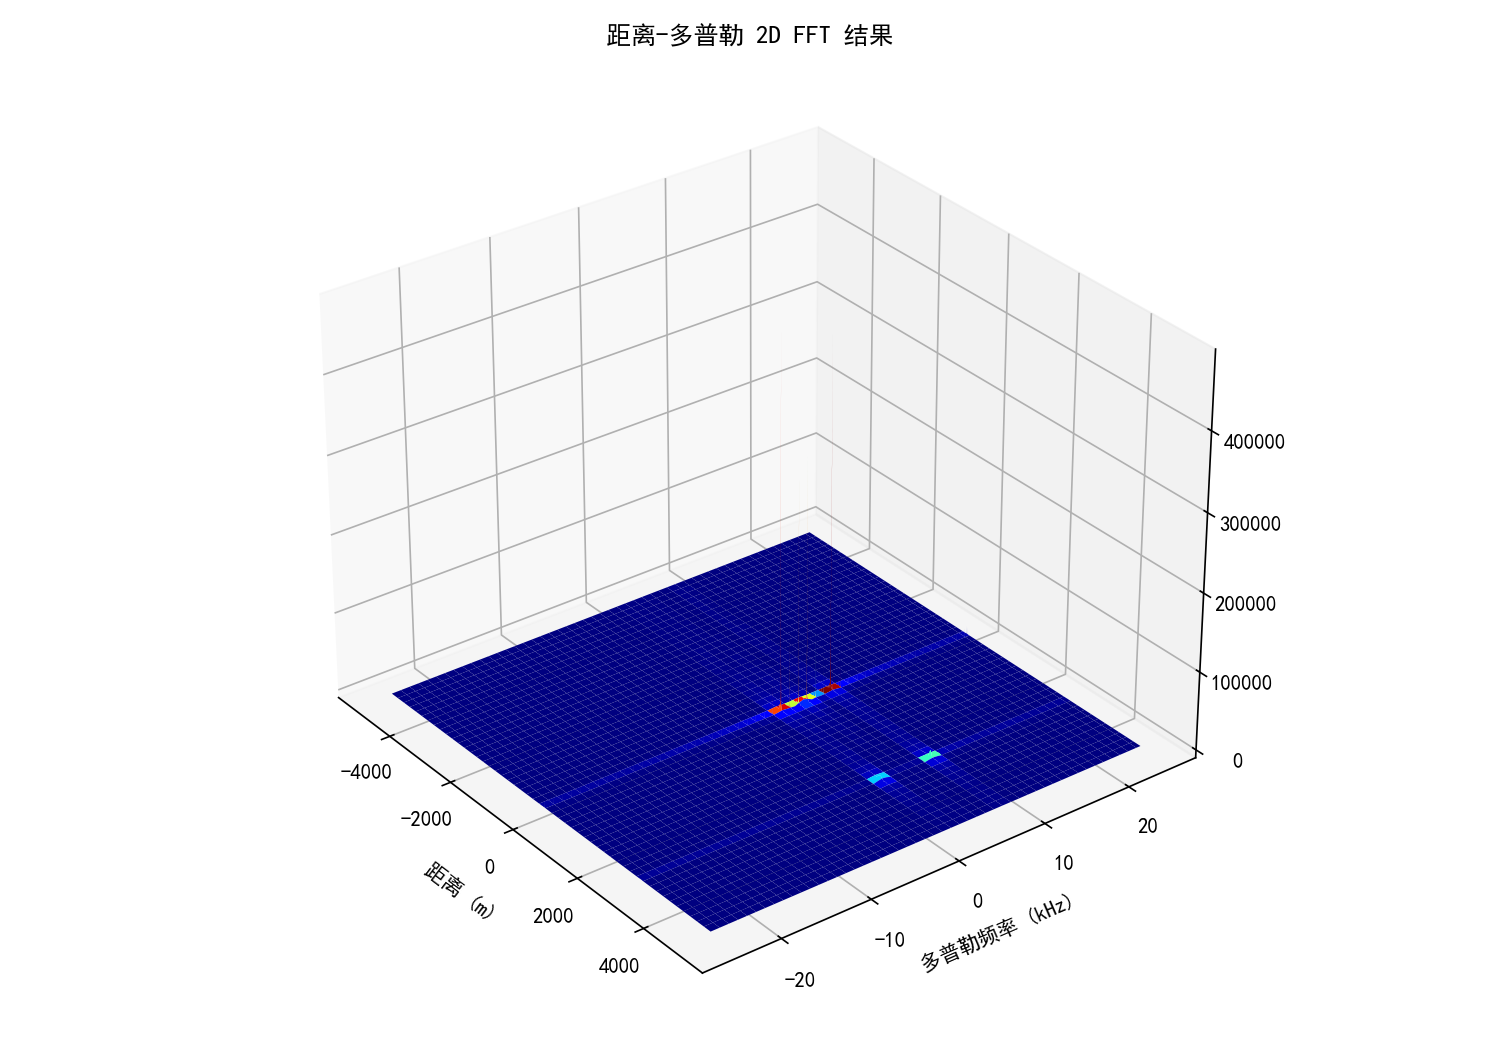
\includegraphics[width=0.85\textwidth]{fig7_range_doppler_mesh.png}
    \caption{距离-多普勒二维 FFT 三维网格图}
    \label{fig:rd_map}
\end{figure}

图 \ref{fig:vel_slice} 为在距离 32 m 处（对应目标1）沿多普勒维的切片，显示目标1的多普勒频率峰值位于约 4.5 kHz 处，与其预设速度一致。

\begin{figure}[H]
    \centering
    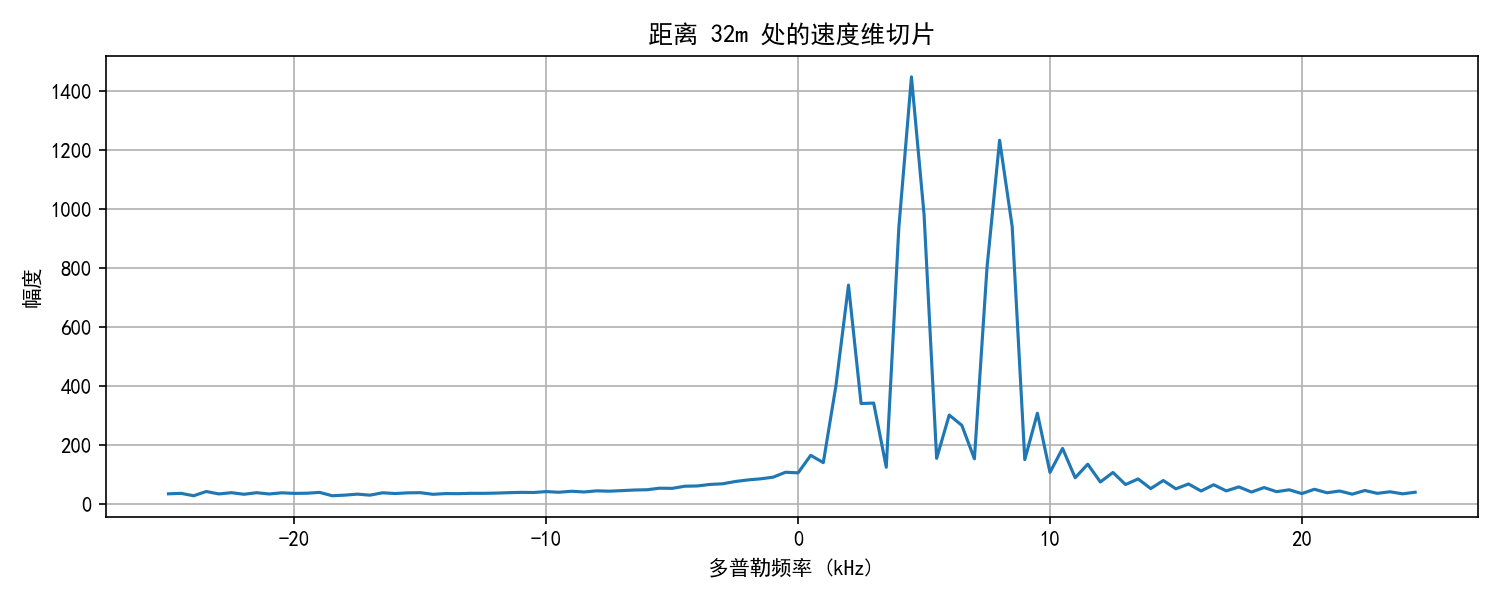
\includegraphics[width=0.85\textwidth]{fig9_velocity_slice_32m.png}
    \caption{距离 32 m 处速度维切片}
    \label{fig:vel_slice}
\end{figure}

\subsection{仿真小结}

仿真结果表明，通过距离维 FFT 和二维 FFT 处理，FMCW 雷达能够有效分辨多个不同距离和速度的目标。三个目标的距离和速度测量值与预设参数完全一致，验证了 FMCW 雷达多目标探测能力的正确性。

% ==================== 第二部分：目标分类 ====================
\section{基于机器学习的雷达目标分类}

\subsection{数据描述}

实测数据为毫米波雷达采集的三类目标的航迹数据，以 MATLAB 的 \texttt{.mat} 格式存储。每类目标的数据概况如下：

\begin{table}[H]
\centering
\caption{实测数据集概况}
\begin{tabular}{lccc}
\toprule
\textbf{目标类别} & \textbf{类别标签} & \textbf{航迹数} & \textbf{轨迹点总数} \\
\midrule
金杯（小型客车） & 0 & 12 & 627 \\
厢式货车（大型货车） & 1 & 17 & 546 \\
无人机 & 2 & 30 & 756 \\
\midrule
\textbf{合计} & — & \textbf{59} & \textbf{1929} \\
\bottomrule
\end{tabular}
\end{table}

每条航迹数据为一个 $N \times 9$ 的矩阵，其中 $N$ 为该航迹包含的轨迹点数，前 8 列为目标在各时刻的雷达特征（包括目标 ID、时间戳、距离、方位角、速度、RCS 等信息），第 9 列为航迹标签。本次分类从中提取了每个轨迹点对应的 7 维特征向量。

\subsection{特征工程}

为了充分利用航迹信息，本实验采用了两种特征构建方式：

\subsubsection{方案A：轨迹点级特征}

直接将每个轨迹点的 7 维特征作为独立样本输入分类器。该方案样本量大（训练集 1350 条，测试集 579 条），但忽略了同一航迹内轨迹点之间的时序关联性。

\subsubsection{方案B：文件级（航迹级）特征}

以每条航迹为单位，对航迹内所有轨迹点的 7 维特征提取统计量（均值、标准差、最大值、最小值），构成 28 维特征向量。该方案样本量较小（训练集 41 条航迹，测试集 18 条航迹），但更能体现整条航迹的整体特性。

\subsection{分类模型}

本实验选用以下四种机器学习模型进行对比：

\begin{itemize}[leftmargin=*]
    \item \textbf{SVM（RBF 核）：} 采用高斯径向基核函数，适用于非线性分类问题。参数设置：$C=10$，$\gamma = \text{scale}$。
    \item \textbf{SVM（线性核）：} 线性支持向量机，适用于线性可分数据。参数设置：$C=1.0$。
    \item \textbf{决策树：} 基于信息增益的树结构分类器。参数设置：最大深度为 5，防止过拟合。
    \item \textbf{随机森林：} 集成学习方法，由 100 棵决策树组成。参数设置：最大深度为 8。
\end{itemize}

所有模型训练前均对特征进行标准化处理（零均值、单位方差），训练集和测试集按 7:3 比例分层划分（保证各类别比例一致）。

\subsection{分类结果与分析}

\subsubsection{方案A：轨迹点级分类}

\begin{table}[H]
\centering
\caption{轨迹点级分类结果}
\begin{tabular}{lcc}
\toprule
\textbf{模型} & \textbf{测试准确率} & \textbf{5折交叉验证准确率} \\
\midrule
SVM (RBF核) & \textbf{98.10\%} & 97.56\% ± 0.65\% \\
随机森林    & 97.58\% & 96.37\% ± 1.23\% \\
SVM (线性核) & 97.41\% & 96.81\% ± 1.11\% \\
决策树      & 94.99\% & 94.22\% ± 1.58\% \\
\bottomrule
\end{tabular}
\end{table}

轨迹点级分类的混淆矩阵如图 \ref{fig:cm_point} 所示。四种模型均取得了较高的分类准确率（均 > 94\%），其中 SVM（RBF 核）表现最佳，达到 98.10\%。这表明单个轨迹点的雷达特征已具有较强的类别区分能力。

\begin{figure}[H]
    \centering
    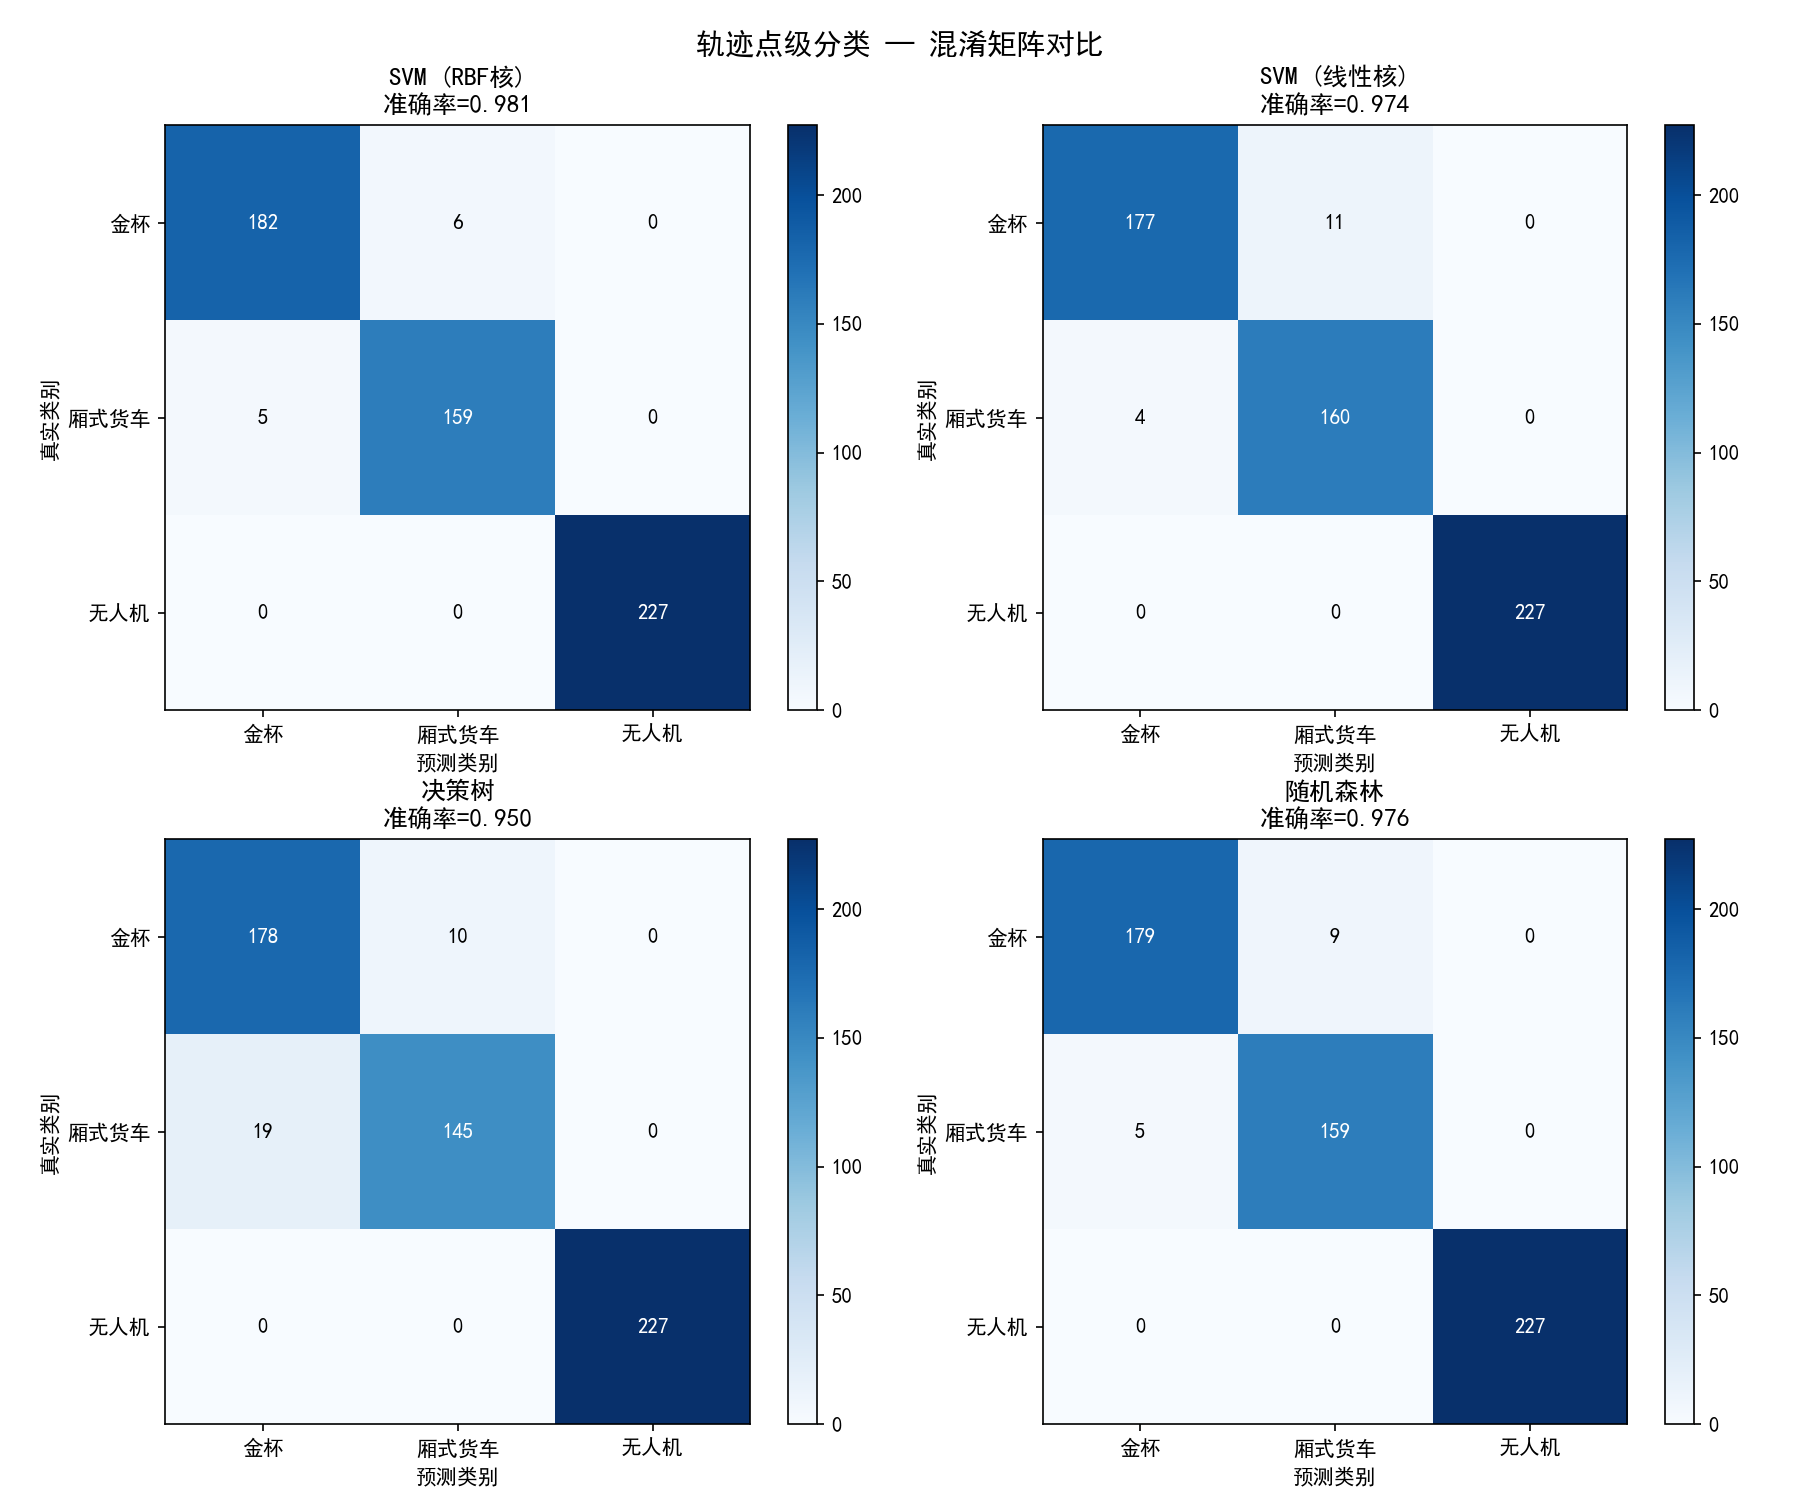
\includegraphics[width=0.90\textwidth]{fig_classification_point_level.png}
    \caption{轨迹点级分类——混淆矩阵对比}
    \label{fig:cm_point}
\end{figure}

\subsubsection{方案B：文件级（航迹级）分类}

\begin{table}[H]
\centering
\caption{文件级（航迹级）分类结果}
\begin{tabular}{lccc}
\toprule
\textbf{模型} & \textbf{测试准确率} & \textbf{5折CV准确率} & \textbf{加权F1分数} \\
\midrule
随机森林    & \textbf{94.44\%} & 100.00\% ± 0.00\% & 0.94 \\
SVM (线性核) & 88.89\% & 100.00\% ± 0.00\% & 0.89 \\
决策树      & 88.89\% & 90.00\% ± 5.00\%  & 0.88 \\
SVM (RBF核) & 83.33\% & 100.00\% ± 0.00\% & 0.82 \\
\bottomrule
\end{tabular}
\end{table}

文件级分类的混淆矩阵如图 \ref{fig:cm_file} 所示。随机森林表现最佳（94.44\%），仅将 1 条金杯航迹误判为厢式货车。值得注意的是，金杯和厢式货车同属于地面车辆，其雷达回波特性有一定相似性，因此在部分模型中出现相互误判。

\begin{figure}[H]
    \centering
    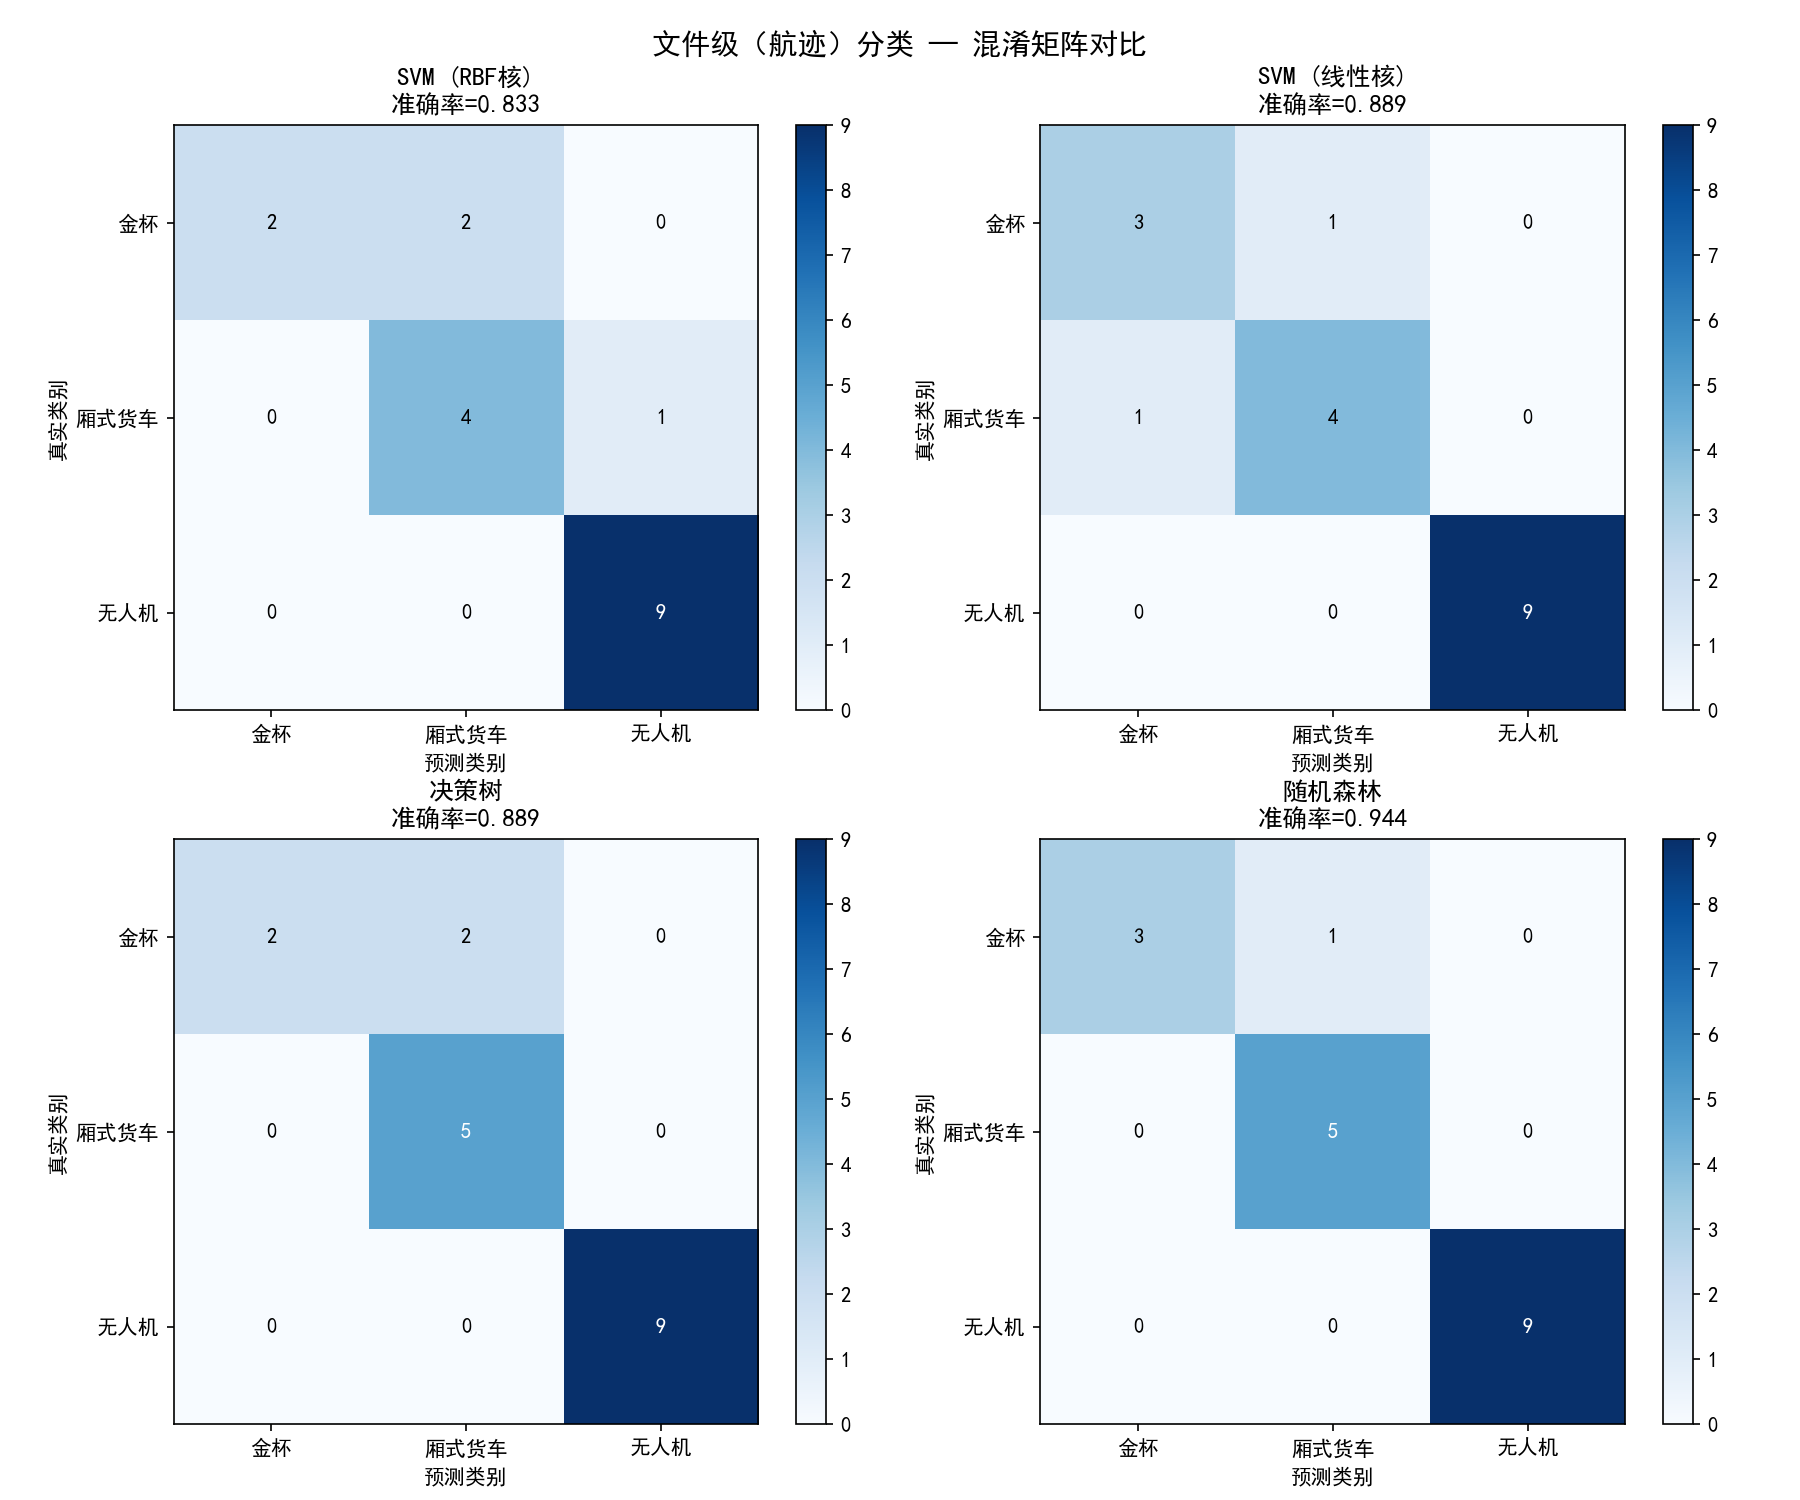
\includegraphics[width=0.90\textwidth]{fig_classification_file_level.png}
    \caption{文件级（航迹级）分类——混淆矩阵对比}
    \label{fig:cm_file}
\end{figure}

\subsection{分类小结}

综合分析两种方案的分类结果：

\begin{enumerate}[leftmargin=*]
    \item \textbf{轨迹点级分类准确率更高}，主要得益于大样本量带来的统计优势。
    \item \textbf{无人机识别效果最好}，在所有模型中均能实现接近 100\% 的识别率，说明无人机的雷达特征与地面车辆存在显著差异（如 RCS 更小、运动模式不同等）。
    \item \textbf{金杯与厢式货车间存在少量混淆}，二者同为地面车辆，在尺寸和运动特征上的相似性导致部分误判。
    \item \textbf{随机森林和 SVM（RBF 核）整体表现最优}，适合作为该分类任务的推荐模型。
\end{enumerate}

% ==================== 总结 ====================
\section{总结}

本报告完成了智能感知技术课程大作业的两项任务：

\textbf{第一部分}成功将 MATLAB 版 FMCW 雷达仿真程序翻译为 Python，并在此基础上添加了两个新目标。仿真结果清晰地展示了三个不同距离（32 m、60 m、85 m）和速度（28.12 m/s、12.50 m/s、50.00 m/s）目标在距离维和距离-多普勒维上的峰值响应，验证了 FMCW 雷达多目标探测的工作原理。

\textbf{第二部分}基于实测雷达数据，采用四种机器学习方法对金杯、厢式货车、无人机三类目标进行分类。轨迹点级分类中 SVM（RBF 核）达 98.10\% 准确率，文件级分类中随机森林达 94.44\% 准确率。结果表明，基于雷达特征的机器学习方法能够有效区分不同类型的目标，特别是无人机与地面车辆的区分效果显著。

\end{document}
